% ==============================================================================
% LAB 167
% MÄTNING PÅ ELEKTRISKA KRETSAR
% --------------------------
% Last updated <2015-03-10> 
%
% Author:
% Jonas Sjöberg     <tel12jsg@student.hig.se>
% Oscar Wallberg    <tco13owg@student.hig.se>
% 
% License:
% Creative Commons Attribution-NonCommercial-ShareAlike 4.0 International
% See LICENSE.md for full licensing information.
% ==============================================================================

% ==============================================================================
% INCLUDES AND CONFIGURATION
% ==============================================================================
\documentclass[11pt,a4paper]{article}
\usepackage[utf8]{inputenc}
\usepackage[swedish]{babel} % För svensk innehållsförteckning
\usepackage{siunitx} % (För dokumentation, kör i terminalen; texdoc siunitx)
\usepackage{amssymb}
\usepackage{amsmath}
\usepackage{amsfonts}
\usepackage{graphicx}
\usepackage{booktabs}
\usepackage{longtable} % Tables span across pages
\usepackage{microtype}
\usepackage{gensymb}
%\usepackage{tabto}
\usepackage{units}

\setlength\parindent{0pt} % Removes all indentation from paragraphs

% ==============================================================================
% DOCUMENT METADATA 
% ==============================================================================
\title{EE466 \\ Lab 167 \\ Mätning på elektriska kretsar}

\author{\\
  Jonas Sjöberg\\
  Högskolan i Gävle,\\
  Elektronikingenjörsprogrammet,\\
  \texttt{tel12jsg@student.hig.se}\\
  \\
  Oscar Wallberg\\
  Högskolan i Gävle,\\
  Dataingenjörsprogrammet,\\
  \texttt{tco13owg@student.hig.se}\\}

\date{}
% ==============================================================================
\begin{document}
% ==============================================================================
\maketitle

\begin{center}
    \begin{tabular}{l r}
        Labb utförd: & ? Februari 2015 \\
        Instruktör: & Efrain Zenteno
    \end{tabular}
\end{center}

% ==============================================================================
% ABSTRACT
% ==============================================================================
\begin{abstract}
    Syftet med laborationen är att praktiskt pröva några av de grundläggande
    sambanden och satserna i likströmsläran, samt att förstå enkla
    växelströmskretsar. Dessutom bör studenten efter genomförd laboration
    översiktligt förstå universalinstrumentets och oscilloskopets principiella
    funktionssätt, samt kunna tillämpa hanteringen av dessa instrument i
    mätning på elektriska kretsar.
\end{abstract}

\newpage

{
    %\hypersetup{linkcolor=black}
    \setcounter{tocdepth}{3}
    \tableofcontents
}

\newpage

% ==============================================================================
% SECTION: INTRODUKTION 
% ==============================================================================
\section{Introduktion}\label{setup}
% ==============================================================================
% TODO: Allmän introduktion.


% ==============================================================================
% SECTION: 1 MÄTNING PÅ SERIESKRETS
% ==============================================================================
\section{Mätning på seriekrets}\label{}
% ==============================================================================
% TODO: Kopplingsschema.

\subsection{Mätresultat}\label{}
% ------------------------------------------------------------------------------
% TODO: + Spänningarna mellan AB, BC och AC.

\subsection{Kommentar}\label{}
% ------------------------------------------------------------------------------
% TODO: Kommentera utgående från Kirchhoffs 2:a lag.
%       Kommentera utgående från spänningsdelningslagen.


% ==============================================================================
% SECTION: 2 iNVERKAN AV EN PARALLELLGREN PÅ EN KRETS
% ==============================================================================
\section{Inverkan av en parallellgren på en krets}\label{}
% ==============================================================================
% TODO: Kopplingsschema.

\subsection{Mätresultat}\label{}
% ------------------------------------------------------------------------------
% TODO: Mät strömmen i punkten B samt strömmen direkt från spänningskällan.


% ==============================================================================
% SECTION: 3 MÄTNING PÅ PARALLELLKRETS
% ==============================================================================
\section{Mätning på parallellkrets}\label{}
% ==============================================================================
% TODO: Kopplingsschema.

\subsection{Mätresultat}\label{}
% ------------------------------------------------------------------------------
% TODO: Mät de markerade strömmarna

\subsection{Kommentar}\label{}
% ------------------------------------------------------------------------------
% TODO: Kommentera utgående från Kirchhoffs 1:a lag.


% ==============================================================================
% SECTION: 4 MÄTNING AV RESISTANS
% ==============================================================================
\section{Mätning av resistans}\label{}
% ==============================================================================
% TODO: Kopplingsschema.

\subsection{Mätresultat}\label{}
% ------------------------------------------------------------------------------
% TODO: Mät resistansen mellan A och B i nedanstående kretsar.

\subsection{Teoretisk beräkning}\label{}
% ------------------------------------------------------------------------------
% TODO: För varje mätning skall du verifiera resultatet med en teoretisk beräkning.

%\subsection{Kommentar}\label{}
% ------------------------------------------------------------------------------
% TODO: Kommentar på skillnader mellan mätresultat och beräkning?


% ==============================================================================
% SECTION: 5 MÄTNING AV EMK OCH INRE RESISTANS I EN TVÅPOL
% ==============================================================================
\section{Mätning av emk och inre resistans i en tvåpol}\label{}
% ==============================================================================
Dessa mätningar görs i syfte att undersöka konceptet tvåpol och reducering av 
komplexa nät med hjälp av Thévenins ekvivalens.
\par En så kallad experimentplatta eller "breadboard" används för att konstruera
kretsen som illustreras i Figur \ref{fig:lab-03_5-schem}. Nätaggregatet \textbf{V1}
är ett strömbegränsande laboratorieaggregat HP3631A.
Spänningen \textbf{U} mäts över dekadresistorn \textbf{R3} med
bänkmultimetern \textbf{M2}, en HP34401A. 
Strömmen \textbf{I} mäts genom att den handhållna multimetern Tenma 72-2050
kopplas mellan punkten \textbf{A} och \textbf{R3}. 

\begin{figure}
\centering
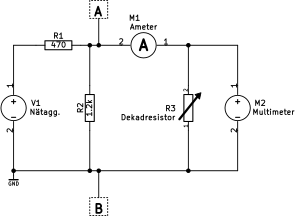
\includegraphics[width=0.7\linewidth]{img/lab-03_5-schem}
\caption[Kopplingsschema för mätning av tvåpol.]
{Schematisk bild av uppkoppling vid mätning av EMK och inre resistans i en tvåpol.}
\label{fig:lab-03_5-schem}
\end{figure}

% TODO: Mät tvåpolens tomgångsspänning, Uab0, d.v.s. ställ Ry på sitt maximala värde.
%       Minska Ry tills spänningen över Ry har minskat till 0.5.Uab0 (d.v.s hälften av
%       tomgångsspänningen).
%
%       * Värdet på Ry då tvåpolens spänning har sjunkit till hälften är lika stort som
%         tvåpolens inre resistans, Ri. Utred varför!
%       * Härled med Thévenins teorem de teoretiska värden på Uab0 och Ri.


% ==============================================================================
% SECTION: 6 KARAKTERISTIK HOS EN LYSDIOD
% ==============================================================================
\section{Karakteristik hos en lysdiod}\label{}
% ==============================================================================
% TODO: Rita grafen I=f(U)! Kommentera!


% ==============================================================================
% SECTION: 7 MÄTNING AV VÄXELSPÄNNING MED UNIVERSALINSTRUMENT OCH OSCILLOSKOP
% ==============================================================================
\section{Mätning av växelspänning med universalinstrument och oscilloskop}\label{}
% ==============================================================================
% TODO


% ==============================================================================
% SECTION: 8 STUDIUM AV FREKVENSGÅNG I EN REAKTIV KRETS
% ==============================================================================
\section{Studium av frekvensgång i en reaktiv krets}\label{}
% ==============================================================================
% TODO: Kopplingsschema.

\subsection{Mätresultat}\label{}
% ------------------------------------------------------------------------------
% TODO: + Gör upp en tabell som för varje frekvens anger
%         - tongeneratorns signalamplitud,
%         - amplituden hos spänningen över den studerade kondensatorn
%         - kvoten mellan den senare amplituden och den tidigare
%         - samt om fasförskjutning förekommer.

\subsection{Teoretisk beräkning}\label{}
% ------------------------------------------------------------------------------
% TODO: Kontrollera dina resultat genom att utnyttja följande formel:

\subsection{Kommentar}\label{}
% ------------------------------------------------------------------------------
% TODO:


% ==============================================================================
% SECTION: 9 MÄTNING AV FASFÖRSKJUTNING I EN REAKTIV KRETS
% ==============================================================================
\section{Mätning av fasförskjutning i en reaktiv krets}\label{}
% ==============================================================================
% TODO: Kopplingsschema.
%       Samma koppling som förra uppgiften, kanske överflödigt att upprepa?

\subsection{Mätresultat}\label{}
% ------------------------------------------------------------------------------
% TODO:

\subsection{Teoretisk beräkning}\label{}
% ------------------------------------------------------------------------------
% TODO: Kontrollera dina resultat genom att utnyttja följande formel:

\subsection{Kommentar}\label{}
% ------------------------------------------------------------------------------
% TODO: Kommentera resultatet


% ==============================================================================
% SECTION: 10 MÄTNING AV RESONANSFREKVENS
% ==============================================================================
\section{Mätning av resonansfrekvens}\label{}
% ==============================================================================
% TODO: Kopplingsschema.

\subsection{Mätresultat}\label{}
% ------------------------------------------------------------------------------
% TODO: Notera resonansfrekvensen. 

\subsection{Kommentar}\label{}
% ------------------------------------------------------------------------------
% TODO: + Kommentera följande:                                                            
%          - Förekommer fasförskjutning mellan uTG och uR vid denna frekvens?
%          - Ändrar fasen sig om du varierar frekvensen kring den
%            uppmätta resonansfrekvensen?  I så fall hur?
%          - Om laboration 61 har gjorts, jämför resultatet med de uppmätta
%            värderna.  Stämmer de överens om inte, varför?


% ==============================================================================
% SECTION: RESULTAT
% ==============================================================================
\section{Resultat}\label{setup}
% ==============================================================================
% TODO: Övergripande resultat/sammanfattning/kommentar på HELA labben.

\newpage

% ==============================================================================
% SECTION: REFERENSER
% ==============================================================================
\section{Referenser}\label{refs}
% ==============================================================================
%TODO: Referenser.

%\subsection{www}\label{interwebs}
% ------------------------------------------------------------------------------

%\subsection{Trycksaker}\label{literature} %???
% ------------------------------------------------------------------------------

%\subsection{Källkod}\label{sourcefiles}
% ------------------------------------------------------------------------------

% ==============================================================================
\end{document}
% ==============================================================================
